\section{Aufbau}
\begin{figure}
  \centering
  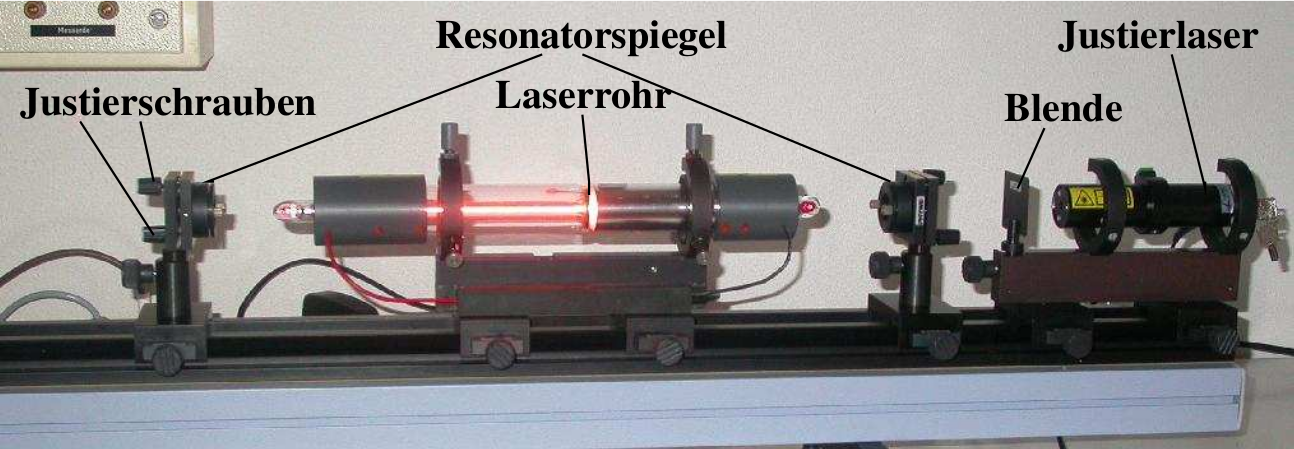
\includegraphics[height = 4cm]{pics/Aufbau.png}
  \caption{Foto des grundlegenden Aufbaus.}
  \label{fig:Aufbau}
\end{figure}
Der wesentliche Aufbau des Versuches ist in der \autoref{fig:Aufbau} zu sehen, dieser besteht aus dem 
Laserrohr und den zwei Spiegeln. Ein Spiegel ist teildurchlässig und spährisch. Der andere Spiegel kann 
ausgewechselt werden, hier wurde ein ebener Spiegel und ein Spiegel mit Krümmungsradius 
$r = \SI{1400}{\milli\meter}$ verwendet. Der teildurchlässige Spiegel hat den gleichen Krümmungsradius. 
Neben dem Laserrohr und den Spiegeln steht ein Laser mit einer Blende, der zur Justage des 
Aufbaues benutzt werden soll. Auf der Blende ist ein Fadenkreuz eingezeichnet. Der ganze Aufbau 
ist auf einer Schiebebahn aufgebracht.\\
\section{Durchführung}
\label{sec:Durchführung}
\paragraph{Justage}
Am Ende der Bahn wird eine Blende angebracht die gleich der vor dem Justierlaser ist. Nun werden 
nach einander die Spiegel und das Laserrohr in den Strahl des Lasers eingebracht und justiert. Das wird 
erreicht in dem der Laserstrahl des Justierlasers auf beiden Blenden genau in der Mitte des 
Fadenkreuzes auftrifft. Sind alle optischen Apparaturen zur optischen Achse justiert, kann das 
Laserrohr in Betrieb genommen werden jetzt müssen die Spiegel noch feinjustiert werden, damit der 
Laseranfängt zu lasen. Ist dieser Teil abgeschlossen können die Messungen begonnen werden.
\paragraph{Bestimmung der Wellenlänge}
Zur Bestimmung der Wellenlänge wird ein Gitter oder ein Spalt in den Strahlengang eingebracht. 
Dann kann mit einer Diode, die auf einem Schlitten senkrecht zur optischen Achse angebracht und 
über eine Mikrometerschraube verschiebbar ist, die Intensitätsverteilung der Beugungsmaxima und -minima 
gemessen werden. Darüber kann dann die Wellenlänge des Lasers bestimmt werden.
\paragraph{Bestimmung der Polarisation}
Die Polarisation wird über einen Polarisator gemessen. Dafür wird die Diode genau in die optische Achse 
gestellt. Dann wird der Winkel des Polarisator variiert und die resultierende Intensität gemessen. 
Das Maximum der Intensitätsverteilung in Abhängigkeit des Polarisationswinkels gibt den 
Polarisationswinkel des Laserlichtes. 
\paragraph{Überprüfung der Stabilitätsbedingung}
Die Stabilitätsbedingung für die verwendeten Spiegel wurden über die Gleichung \eqref{eq:osF} bestimmt 
und in der Abbildung \ref{fig:Stabi} dargestellt. Nun soll der Resonator so weit vergrößert werden, 
bis sich die Laserfähigkeit einstellt. Da die optische Apparatur nicht immer genau zur optischen 
Achse justiert ist, muss bei der Verschiebung teilweise nachjustiert werden, um die Laserfähigkeit 
bei der Verschiebung zu erhalten.  
\FloatBarrier
\begin{figure}
 \begin{subfigure}{.48\textwidth}
  \centering
  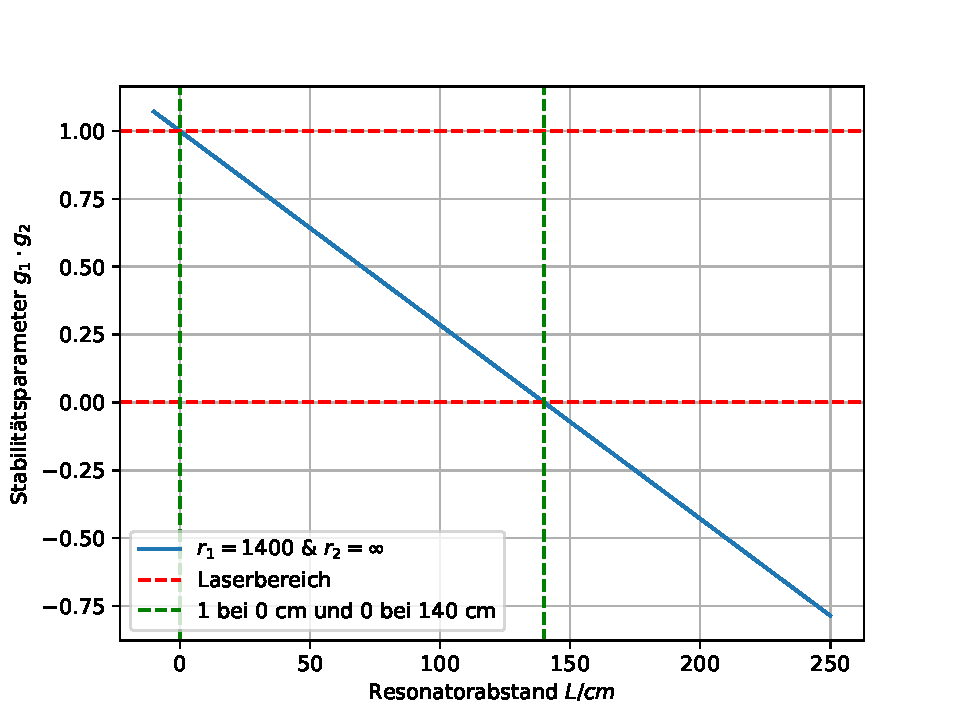
\includegraphics[width = \textwidth]{plots/Vorbereitungsplot1.pdf}
  \caption{zwei sphärische Spiegel.}
  \label{fig:SSS}
\end{subfigure}
\begin{subfigure}{.48\textwidth}
  \centering
  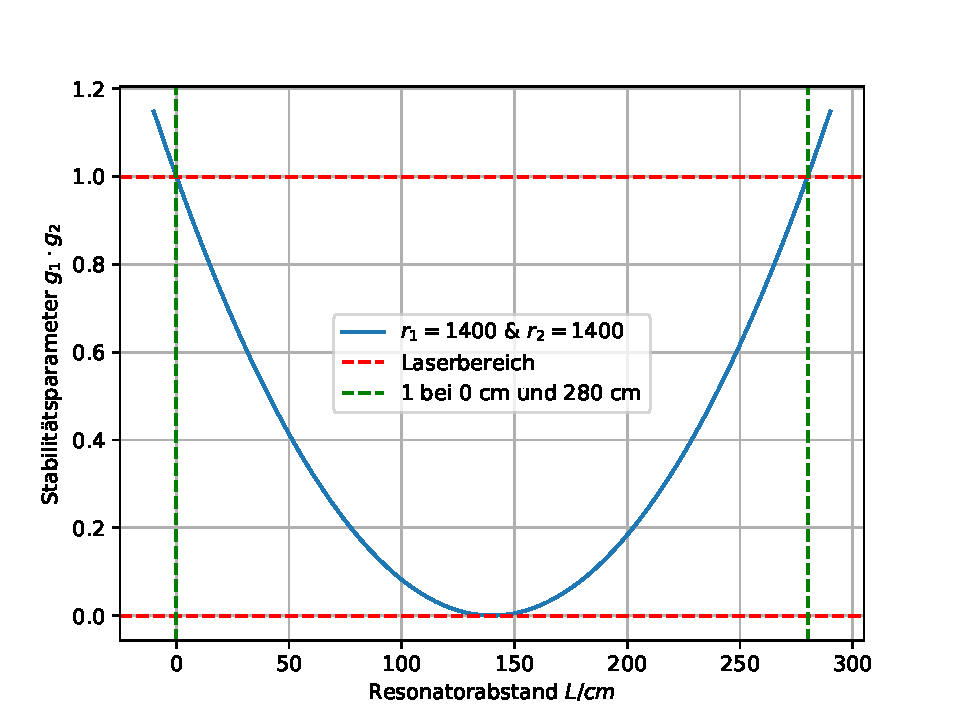
\includegraphics[width = \textwidth]{plots/Vorbereitungsplot2.pdf}
  \caption{einen sphärischen und einen ebenen Spiegel.}
  \label{fig:SSE}
\end{subfigure}
\caption{Stabilitätsbedingung für}
  \label{fig:Stabi}
\end{figure}
\FloatBarrier
\paragraph{Vermessung der TEM-Moden} 
Zuerst kann die TEM$_{000}$-Mode gemessen werden in dem mit einer Diode die Intensitätsverteilung 
des grundlegenden Aufbaus vermessen wird. 
Zur Vermessung weiterer TEM-Moden wird zwischen dem teildurchlässigem Spiegel und dem Laserrohr 
ein Wolframdraht $(d= \SI{0.005}{\milli\meter})$ eingebracht. Der Draht führt dazu das die 
TEM$_{000}$-Mode ausgeblendet wird. Auch hier wird die resultierende Intensitätsverteilung wieder 
mit einer Diode gemessen. 
\paragraph{Vermessung der Schwebung zwischen den longitudinal Moden}
Die longitudinalen Moden können vermessen werden in dem drei verschiedene Resonatorlängen 
eingestellt werden und jeweils der austretende Licht mit einer Diode vermessen wird, die an einen 
Spektrograf angeschlossen ist. Damit kann das Frequenzspektrum, dass bei einer gegebenen Resonatorlänge 
austritt gemessen werden.  

